% ======================================================================
% Questions that simple quiz tools find hard (SAMPLE questions)
% Formulas, matrices, charts, pictures as choices, diagrams, code to trace,
% and numbers that change on every copy.
% Used by the sitting ../types/. See guide/08-question-types-and-scoring.md.
%
% Groups:  types_rich          (one correct answer each)
%          types_random_num    (number answer, different numbers per copy)
% ======================================================================

% ----------------------------------------------------------------------
% Formulas in the question and in the choices
% ----------------------------------------------------------------------
\element{types_rich}{
\begin{question}{RICH001}
What is the value of
\[ \int_0^1 2x\,dx \;+\; \sum_{k=1}^{3} k \; ? \]
\begin{choices}
  \correctchoice{$7$}
  \wrongchoice{$6$}
  \wrongchoice{$8$}
  \wrongchoice{$\tfrac{13}{2}$}
\end{choices}
\end{question}
}

% ----------------------------------------------------------------------
% A matrix product, with matrices as choices
% ----------------------------------------------------------------------
\element{types_rich}{
\begin{question}{RICH002}
Which is the product
$\begin{pmatrix} 1 & 2 \\ 3 & 4 \end{pmatrix}
 \begin{pmatrix} 1 \\ 1 \end{pmatrix}$?
\begin{choices}
  \correctchoice{$\begin{pmatrix} 3 \\ 7 \end{pmatrix}$}
  \wrongchoice{$\begin{pmatrix} 4 \\ 6 \end{pmatrix}$}
  \wrongchoice{$\begin{pmatrix} 1 & 2 \\ 3 & 4 \end{pmatrix}$}
  \wrongchoice{$\begin{pmatrix} 2 \\ 3 \end{pmatrix}$}
\end{choices}
\end{question}
}

% ----------------------------------------------------------------------
% Read a chart drawn in the question
% ----------------------------------------------------------------------
\element{types_rich}{
\begin{question}{RICH003}
The chart shows a shop's sales per quarter. Between which two quarters did sales rise the most?

\begin{center}
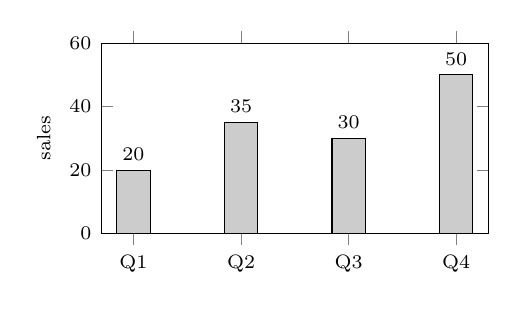
\begin{tikzpicture}
\begin{axis}[ybar, width=6.5cm, height=4cm, bar width=12pt,
    symbolic x coords={Q1,Q2,Q3,Q4}, xtick=data, ymin=0, ymax=60,
    ylabel={sales}, nodes near coords, every node near coord/.style={font=\scriptsize},
    tick label style={font=\scriptsize}, label style={font=\scriptsize}]
  \addplot[fill=gray!40] coordinates {(Q1,20) (Q2,35) (Q3,30) (Q4,50)};
\end{axis}
\end{tikzpicture}
\end{center}
\begin{choices}
  \wrongchoice{Q1 to Q2}
  \wrongchoice{Q2 to Q3}
  \correctchoice{Q3 to Q4}
  \wrongchoice{Sales did not rise}
\end{choices}
\end{question}
}

% ----------------------------------------------------------------------
% Pictures as choices
% ----------------------------------------------------------------------
\newcommand{\MiniScatter}[1]{%
  \begin{tikzpicture}[baseline=1ex, scale=0.32]
    \draw (0,0) rectangle (4,3);
    \foreach \x/\y in {#1} \fill (\x,\y) circle (2.2pt);
  \end{tikzpicture}}

\element{types_rich}{
\begin{question}{RICH004}
Which scatter plot shows a negative correlation?
\begin{choices}
  \correctchoice{\MiniScatter{0.5/2.6, 1.2/2.2, 1.9/1.9, 2.6/1.2, 3.4/0.6}}
  \wrongchoice{\MiniScatter{0.5/0.5, 1.2/1.0, 1.9/1.5, 2.6/2.1, 3.4/2.6}}
  \wrongchoice{\MiniScatter{0.5/1.5, 1.2/1.6, 1.9/1.4, 2.6/1.5, 3.4/1.6}}
  \wrongchoice{\MiniScatter{0.5/2.5, 1.2/0.6, 1.9/2.0, 2.6/0.9, 3.4/2.2}}
\end{choices}
\end{question}
}

% ----------------------------------------------------------------------
% A network diagram
% ----------------------------------------------------------------------
\element{types_rich}{
\begin{question}{RICH005}
The numbers are travel times in minutes. What is the shortest time from A to D?

\begin{center}
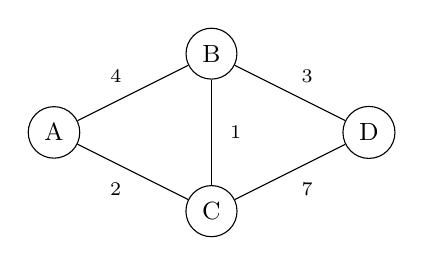
\begin{tikzpicture}[every node/.style={circle, draw, minimum size=6mm, font=\small},
                    every edge/.style={draw}, >=stealth]
  \node (A) at (0,0) {A};
  \node (B) at (2,1) {B};
  \node (C) at (2,-1) {C};
  \node (D) at (4,0) {D};
  \path (A) edge node[draw=none, above left, font=\scriptsize] {4} (B)
        (A) edge node[draw=none, below left, font=\scriptsize] {2} (C)
        (C) edge node[draw=none, right, font=\scriptsize] {1} (B)
        (B) edge node[draw=none, above right, font=\scriptsize] {3} (D)
        (C) edge node[draw=none, below right, font=\scriptsize] {7} (D);
\end{tikzpicture}
\end{center}
\begin{choices}
  \correctchoice{6 minutes}
  \wrongchoice{7 minutes}
  \wrongchoice{9 minutes}
  \wrongchoice{5 minutes}
\end{choices}
\end{question}
}

% ----------------------------------------------------------------------
% A Venn diagram with a shaded region
% ----------------------------------------------------------------------
\element{types_rich}{
\begin{question}{RICH006}
Which set is shaded?

\begin{center}
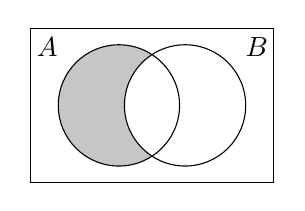
\begin{tikzpicture}[scale=0.7]
  \begin{scope}
    \clip (0,0) circle (1.1);
    \fill[gray!45] (-2,-2) rectangle (3,2);
    \fill[white] (1.2,0) circle (1.1);
  \end{scope}
  \draw (0,0) circle (1.1);
  \draw (1.2,0) circle (1.1);
  \node at (-1.3,1.05) {$A$};
  \node at (2.5,1.05) {$B$};
  \draw (-1.6,-1.4) rectangle (2.8,1.4);
\end{tikzpicture}
\end{center}
\begin{choices}
  \correctchoice{$A \setminus B$}
  \wrongchoice{$A \cap B$}
  \wrongchoice{$A \cup B$}
  \wrongchoice{$B \setminus A$}
\end{choices}
\end{question}
}

% ----------------------------------------------------------------------
% Trace a short program (typeset lines, not a verbatim block: verbatim
% does not work inside \element)
% ----------------------------------------------------------------------
\element{types_rich}{
\begin{question}{RICH007}
What does this program print?

\begin{center}
\begin{tabular}{@{}r@{\quad}l@{}}
\scriptsize 1 & \texttt{total = 0} \\
\scriptsize 2 & \texttt{for i in 1, 2, 3, 4:} \\
\scriptsize 3 & \texttt{\ \ \ \ if i is even: total = total + i} \\
\scriptsize 4 & \texttt{print(total)} \\
\end{tabular}
\end{center}
\begin{choices}
  \correctchoice{6}
  \wrongchoice{4}
  \wrongchoice{10}
  \wrongchoice{2}
\end{choices}
\end{question}
}

% ----------------------------------------------------------------------
% Different numbers on every copy, one correct answer.
% \pgfmathrandominteger picks a number; the layout fixes the random seed,
% so the exam, the answer key and the marking all get the same numbers.
% Each wrong choice is a typical mistake, and all four are always
% different (a is 3-9 and b is 11-19, so a+b is always below a*b-b).
% ----------------------------------------------------------------------
\element{types_rich}{
\begin{question}{RICH008}
\pgfmathrandominteger{\RichA}{3}{9}
\pgfmathrandominteger{\RichB}{11}{19}
\pgfmathtruncatemacro{\RichRight}{\RichA*\RichB}
\pgfmathtruncatemacro{\RichSum}{\RichA+\RichB}
\pgfmathtruncatemacro{\RichMore}{\RichA*\RichB+\RichA}
\pgfmathtruncatemacro{\RichLess}{\RichA*\RichB-\RichB}
A student buys \RichA\ notebooks at \RichB\ baht each. How much does the student pay?
\begin{choices}
  \correctchoice{\RichRight\ baht}
  \wrongchoice{\RichSum\ baht}
  \wrongchoice{\RichMore\ baht}
  \wrongchoice{\RichLess\ baht}
\end{choices}
\end{question}
}

% ----------------------------------------------------------------------
% Different numbers on every copy, number answer.
% The three numbers are m-d, m, m+d, so the mean is always the whole number m.
% ----------------------------------------------------------------------
\element{types_random_num}{
\begin{questionmultx}{RICH101}
\pgfmathrandominteger{\RichM}{12}{48}
\pgfmathrandominteger{\RichD}{2}{9}
\pgfmathtruncatemacro{\RichLo}{\RichM-\RichD}
\pgfmathtruncatemacro{\RichHi}{\RichM+\RichD}
What is the mean of \RichHi, \RichLo\ and \RichM?
\AMCnumericChoices{\RichM}{digits=2,sign=false,scoreexact=1}
\end{questionmultx}
}
